\chapter{Laboratórne overenie funkčnosti}

V tejto kapitole predstavíme vlastnosti nami skonštruovaného robota pri laboratórnych testoch. Zameriame sa prevažne na správanie sa robota v režimoch statického balansovania a jeho schopnosť presúvať sa po šikmých plochách.

Pri režime statického balansovania na mieste sa zameriame na priemernú odchýlku od nulového náklonu, amplitúdu oscilácií a celkovú prejdenú vzdialenosť (so zaradením PIDu C aj bez neho).

Všetky grafy požité v tejto kapitole boli vytvorené s použitím nami napísaného python scriptu a dáta v nich zobrazené boli získané prostredníctvom sériovej komunikácie medzi počítačom a robotom.  

\section{Základné parametre robota}
Pre nami vytvoreného robota sme namerali nasledujúce parametre. Tie by mali byť dostatočné pre vytvorenie jednoduchého matematického modelu tohto robota.

\begin{multicols}{2}
\begin{itemize}
\item{$R = 7,2 ~\Omega$}
\item{$K_e = 3,34x10^{-1}$}
\item{$K_m = 9,3x10^{-2}$}
\item{$J_k = 1,598x10^{-3}~ kgm^{2}$}
\item{$J_s = 4,025x10^{-2}~ kgm^{2}$}
\item{$r = 3,4x10^{-2}~ m$}
\item{$m_k = 4,7x10^{-2}~ kg$ss}
\item{$m_p = 1,07 ~kg$}
\item{$L = 0,145 ~m$}
\end{itemize}
\end{multicols}

Pri meraní zotrvačnosti kolesa sme použili vzorec \ref{eq:J_wheel}:
\begin{equation}
J_k = m_kr^2
\label{eq:J_wheel}
\end{equation}

a pre zotrvačnosť celého robota:
\begin{equation}
J_s = \dfrac{m_pgLT^2}{4\pi^2}
\label{eq:J_robot}
\end{equation}
kde $T$ je perióda oscilácie robota okolo osi kolies po vychýlení o malý uhol.


\section{Parametre robota pri balansovaní na mieste}
Pri balansovaní na mieste môže užívateľ zvoliť z dvoch režimov prevádzky. V prvom režime robot balansuje bez toho aby sa snažil udržať počiatočnú pozíciu, v druhom sleduje celkovú prejdenú vzdialenosť a snaží sa ju udržať na minime. Druhý stav je výhodný najmä v prípade ak sa robot nachádza na naklonenej plošine, kde mu sledovanie prejdenej vzdialenosť umožňuje pridávať rýchlosť natoľko aby sa udržal v nehybnosti.

Testovanie správania robota prebiehalo po pripojení k počítaču dlhým, flexibilným káblom, ktorý nám umožnil komunikáciou cez sériovú linku zhromaždiť údaje o stave robota v jednotlivých časových okamihoch. Pomocou týchto dát boli následne vytvorené grafy zobrazené na  \figurename~\ref{fig:combination}. Na osi Y sa nachádzajú odchýlky od pravého uhla pre jednotlivé sledované vzorky. Čas medzi jednotlivými vzorkami bol $t_vz = 50ms$, čiže celkový časový interval, počas ktorého sme sledovali správanie robota trval 50 sekúnd.



\begin{figure}[h]
\centering
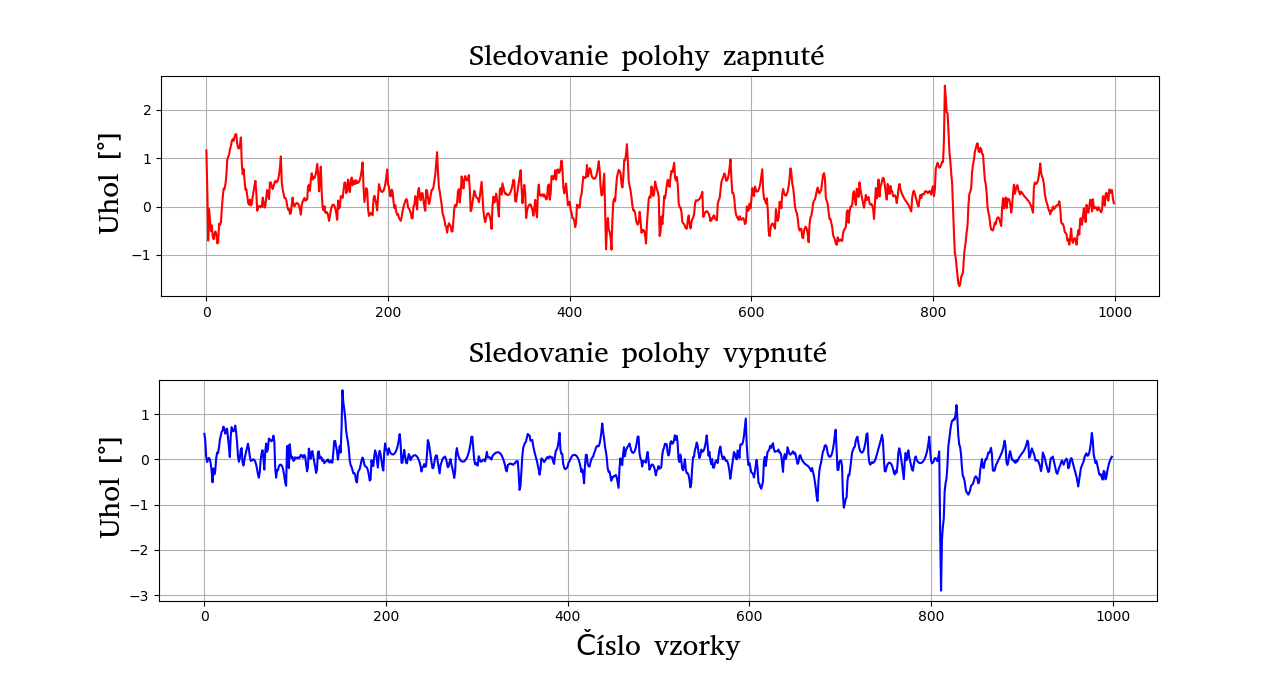
\includegraphics[width=16cm]{combination}
\caption{Náklon robota v čase}
\label{fig:combination}
\end{figure}   

Z porovnania grafov na \figurename~\ref{fig:combination} je zrejmé, že pri vypnutom sledovaní polohy bol robot schopný presnejšie regulovať uhlovú odchýlku od pravého uhla. V tomto režime odchýlka málokedy prekročila hodnotu 1°, čo sa nedá povedať o režime, v ktorom bolo zapnuté sledovanie polohy. Nevýhodou ale bolo, že aj za relatívne krátky čas merania došlo k posunu robota o viac než $5~cm$ oproti počiatočnej polohe, čo v prípade merania v druhom režime nebol problém. Pri sledovaní polohy vzdialenosť robota od počiatočnej polohy nikdy výrazne neprekročila $5~cm$ pričom mal vždy robot tendenciu vracať sa do počiatočnej polohy a oscilovať okolo nej \figurename~\ref{fig:zmena_polohy}.
 
\begin{figure}[h!]
\centering
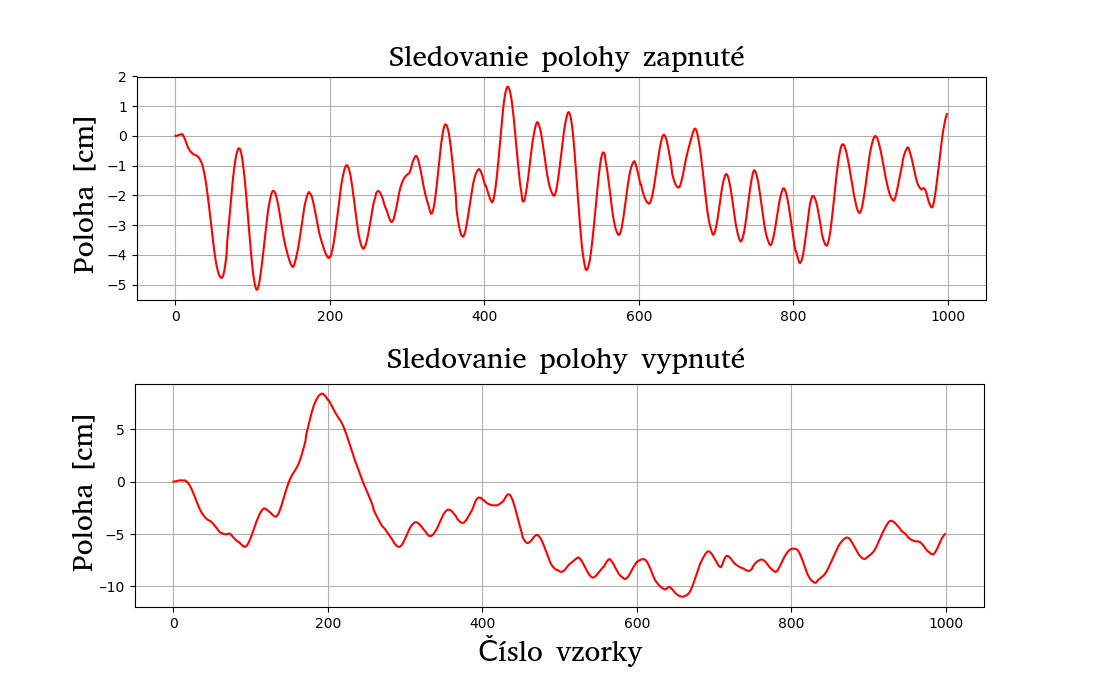
\includegraphics[width=16cm, height=7cm]{zmena_polohy}
\caption{Zmena polohy robota počas testu}
\label{fig:zmena_polohy}
\end{figure}   

Okrem balansovania na rovine sme testovali aj správanie robota pri balansovaní na naklonenej rovine, ktorej sklon bol 15°. Pri tomto teste bol trvalo zapnutý režim so sledovaním polohy keďže, ako už bolo spomenuté, robot nebol bez neho schopný ani zotrvať na plošine. 

Z tohto testu podľa očakávania vyplynulo, že robot vykazoval pri takomto balansovaní zhoršené vlastnosti oproti pohybu na rovine. Oscilácie okolo počiatočného bodu boli väčšie, robot bol však naďalej schopný zotrvať v okolí počiatočnej pozície. Toto ale platilo len pre pohyb v smere náklonu plošiny. Keďže servo pohon nebol v čase písania tejto práce ešte zakomponovaný do riadenia robota, nebol schopný nakloniť šasi tak, aby ostal robot stabilný aj pri pohybe priečnom voči uhlu náklonu plošiny. Tento nedostatok sa prejavoval nerovnomerným pohybom robota, hlavne pri náhlych smeroch jazdy.  

